\documentclass[11pt,a4paper]{article}
\usepackage[hmargin=2cm, vmargin=1.5cm]{geometry}
\usepackage{amsmath,amssymb}
\usepackage{graphicx}
\usepackage{hyperref}

\newcommand{\norm}[1]{\left\| #1 \right\|}
\newcommand{\ip}[2]{\left\langle #1, #2 \right\rangle}

\title{GD, SGD and Polyak stepsizes for logistic regression on the California housing data}
\author{Gor Melkumyan}
\date{}

\begin{document}
\maketitle

\section*{Idea}

After the linear regression, I repeat the same experiments with a model that cannot be solved exactly: the
logistic regression. Of course, the solution can be found with some approximations, which I used as well, but I
wanted to use another model without overcomplicating things and to concentrate on GD, so I use this one.
There is no formula for the solution $w^\star$, so we compute it once with Newton's method, to machine precision. GD and SGD do not use it; it is only the reference for the error
$\norm{w^k - w^\star}^2$ and gives $f^\star$ for the Polyak stepsize.

\section*{Data and model}

We take the same California house prices data and the same features as before (the logarithm of some of the
features, and the outliers clipped to $[-3, 3]$), but now the task is a classification: a district is
``expensive'' ($y_i = +1$) if its median house value is above the median of the training set, and $y_i = -1$
otherwise. We minimize the logistic loss with a small $\ell_2$ term,
\[
  f(w) = \frac{1}{n}\sum_{i=1}^n f_i(w), \qquad
  f_i(w) = \log\bigl(1 + e^{-y_i\ip{x_i}{w}}\bigr) + \frac{\lambda}{2}\norm{w}^2, \qquad \lambda = 0.01 .
\]
The $\ell_2$ term is needed to make $f$ strongly convex.

\paragraph{The constants.} With $z_i = y_i\ip{x_i}{w}$ and the sigmoid $\sigma(t) = \frac{1}{1+e^{-t}}$, the gradient
and the Hessian of $f_i$ are
\[
  \nabla f_i(w) = -y_i\,\sigma(-z_i)\,x_i + \lambda w, \qquad
  \nabla^2 f_i(w) = \sigma(z_i)\bigl(1 - \sigma(z_i)\bigr)\,x_ix_i^\top + \lambda I .
\]
With $p = \sigma(z_i) \in (0,1)$ we have
$p(1-p) = \frac{1}{4} - \bigl(p - \frac{1}{2}\bigr)^2 \le \frac{1}{4}$, with equality only for $z_i = 0$, i.e.\ when the
model is completely unsure about the point $x_i$.
\begin{itemize}
  \item $L_i$: the matrix $x_ix_i^\top$ has the eigenvalue $\norm{x_i}^2$ in the direction $x_i$ and $0$ in all the
    other directions, so the largest eigenvalue of $\nabla^2 f_i(w)$ is at most $\frac{\norm{x_i}^2}{4} + \lambda$.
    It is attained when $z_i = 0$ (for example at $w = 0$), hence $L_i = \frac{\norm{x_i}^2}{4} + \lambda$.
  \item $L$: the Hessian of $f$ is the average $\frac{1}{n}\sum_i \sigma(z_i)\bigl(1-\sigma(z_i)\bigr)x_ix_i^\top + \lambda I$.
    Bounding every factor by $\frac{1}{4}$ gives $L \le \lambda_{\max}\bigl(\frac{1}{4n}X^\top X\bigr) + \lambda$, and at
    $w = 0$ all the factors are exactly $\frac{1}{4}$, so $L = \lambda_{\max}\bigl(\frac{1}{4n}X^\top X\bigr) + \lambda$.
    As for the linear regression, $L$ is smaller than the average $\bar L = \frac{1}{n}\sum_i L_i$, because the
    directions $x_i$ are different.
  \item $\mu$: the factor $\sigma(1-\sigma)$ is positive, but it tends to $0$ far from the data (when the model is
    very confident), so the only lower bound for all $w$ is $\nabla^2 f(w) \succeq \lambda I$, hence $\mu = \lambda$.
    Without the $\ell_2$ term we would have $\mu = 0$.
\end{itemize}
For our data $\mu = 0.01$, $L = 0.519$, $\bar L = 1.98$ and $L_{\max} = 11.34$, so $A = 2L_{\max} = 22.7$ for SGD-US
and $A_{\rm IS} = 2\bar L = 3.96$ for SGD-IS. These are worst-case constants.

All methods use one target: $\norm{w^k - w^\star}^2 \le 10^{-2}\norm{w^0 - w^\star}^2$.

The code is the file
\href{https://github.com/Gor-2001/thesis_hw/blob/main/Homework/Exercises/hw_2026_11_11/sgd_logistic.ipynb}{\texttt{Homework/Exercises/hw\_2026\_11\_11/sgd\_logistic.ipynb}}.

\section*{Experiments}

The first experiment is GD with the constant stepsize $\frac{1}{L}$.

\begin{center}
  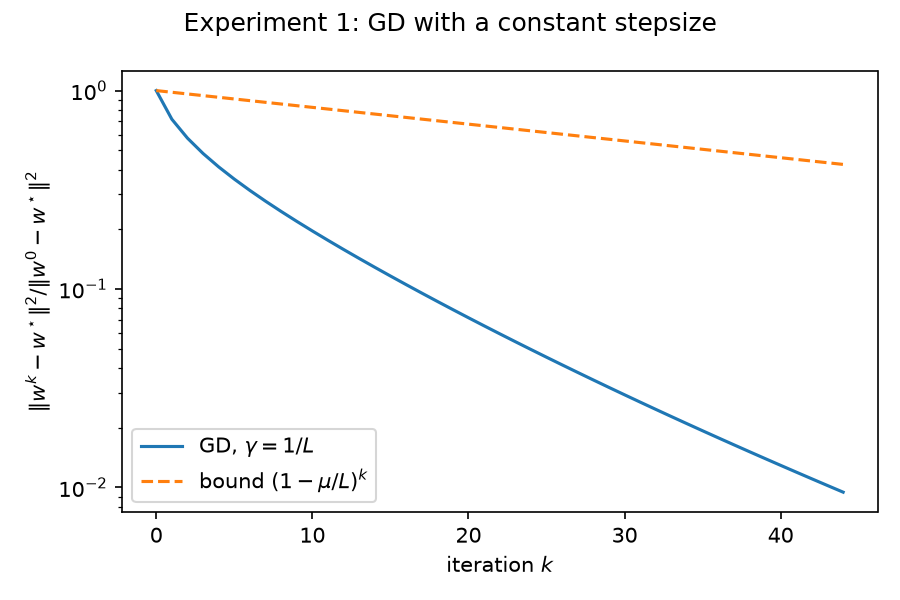
\includegraphics[width=0.6\textwidth]{figures/log_exp1_gd.png}
\end{center}

The second one is GD with the Polyak stepsize, again with the theoretical bounds and the comparison with the
simple GD. Here the Polyak stepsize helps even more than for the linear regression, because it adapts to the
actual curvature, which is much smaller near $w^\star$ than the worst case $L$.

\begin{center}
  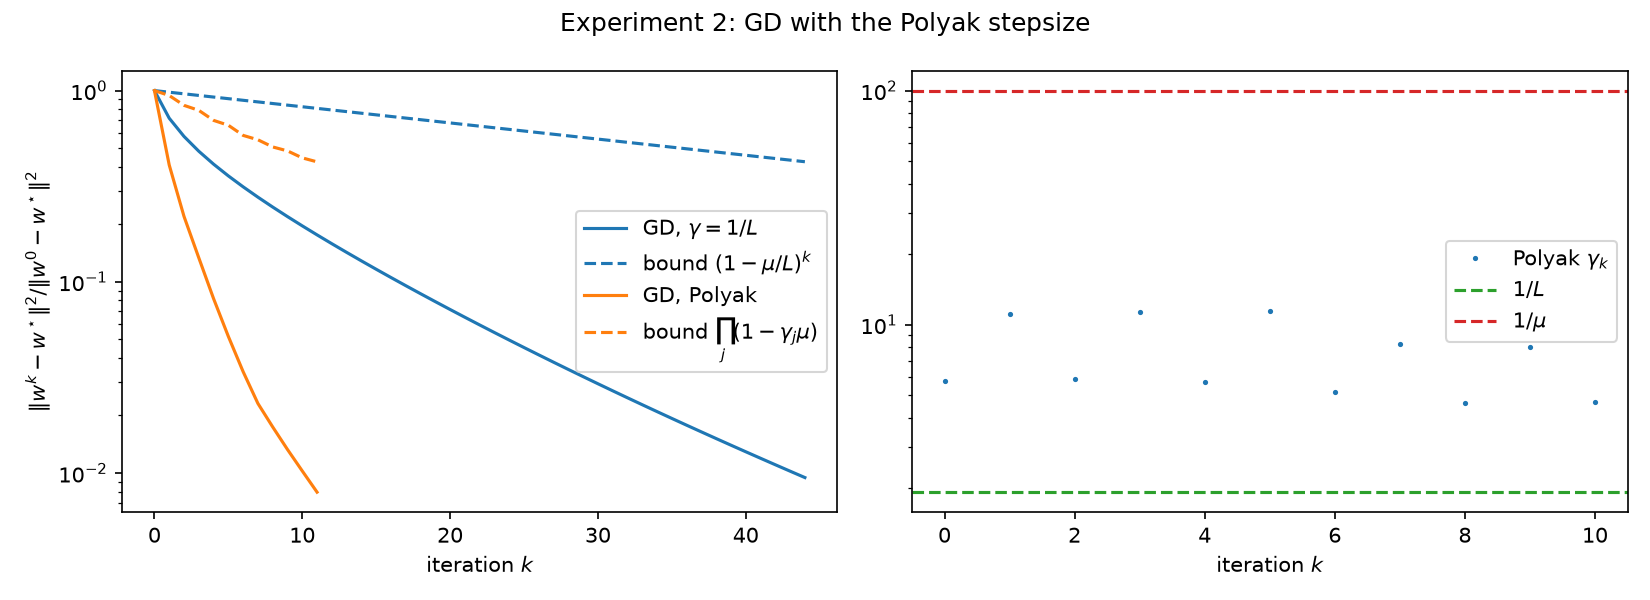
\includegraphics[width=\textwidth]{figures/log_exp2_polyak.png}
\end{center}

After them come SGD-US and SGD-IS with their theoretical maximal stepsizes $\frac{1}{A}$ and with other stepsizes.
Unlike the linear regression, a much larger $\gamma$ than allowed does not make SGD diverge, since the gradients
of the logistic loss are bounded; the method only settles in a much larger neighbourhood.

\begin{center}
  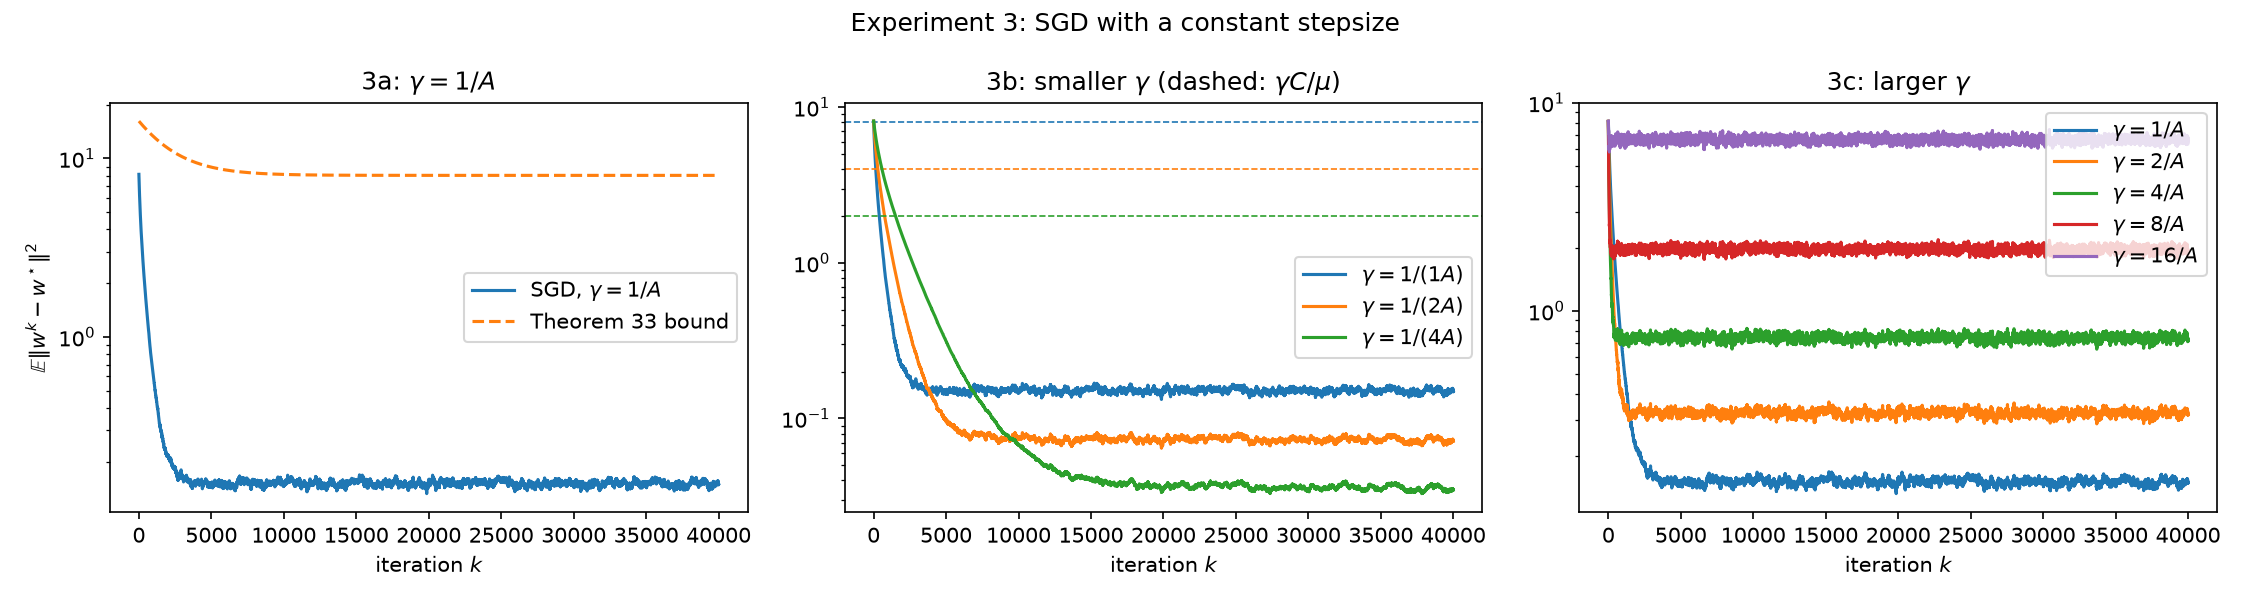
\includegraphics[width=\textwidth]{figures/log_exp3_sgd.png}
\end{center}

\begin{center}
  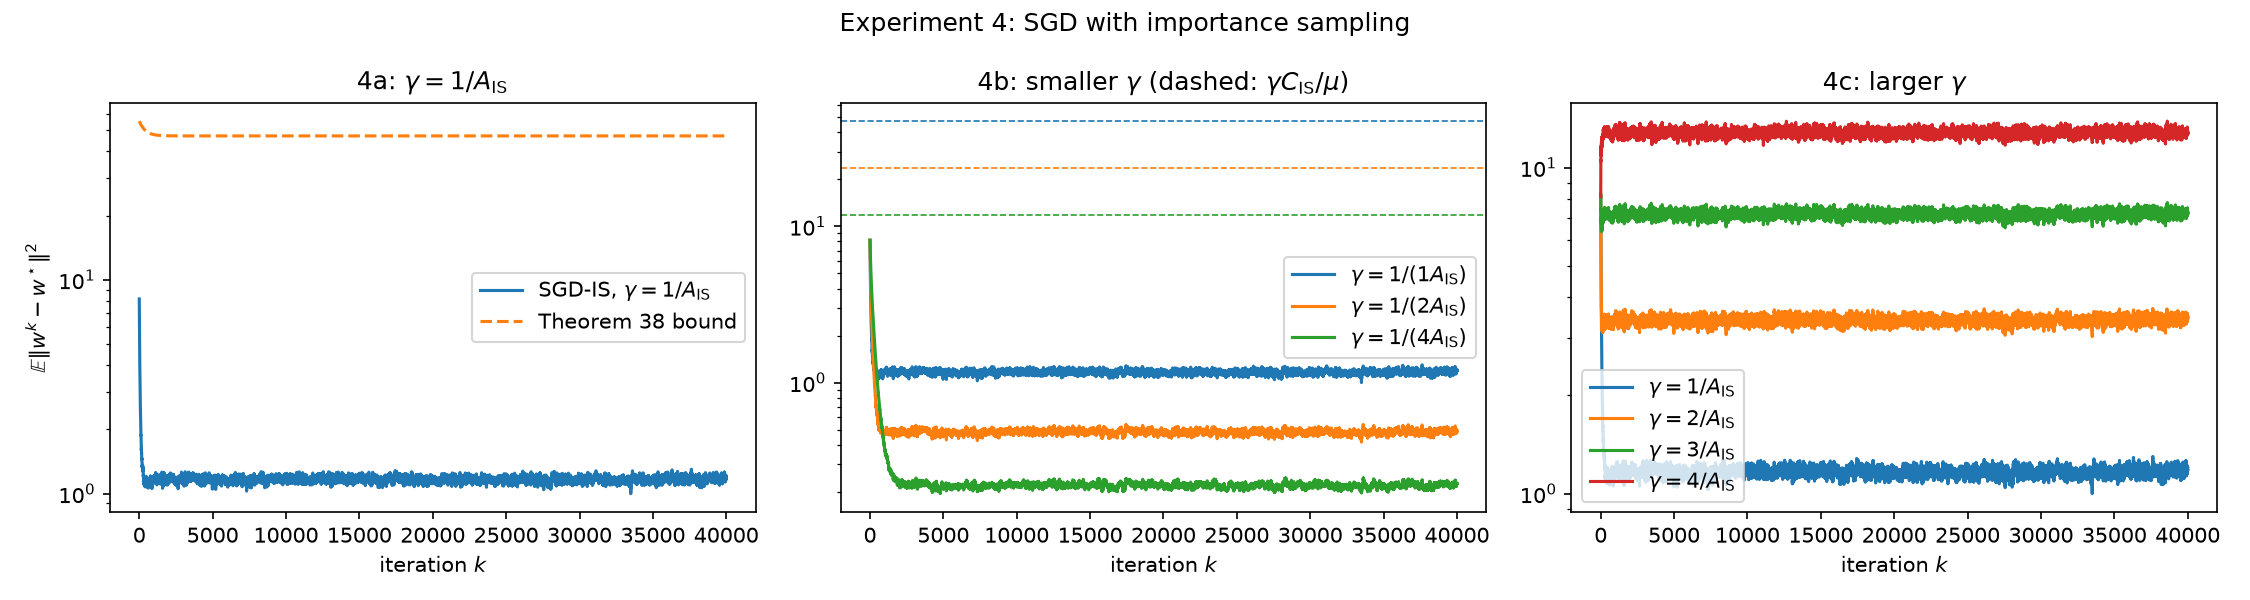
\includegraphics[width=\textwidth]{figures/log_exp4_sgd_is.png}
\end{center}

\section*{Comparison}

The last experiment is the comparison of all the methods, both by the number of iterations and by the time.

\begin{center}
  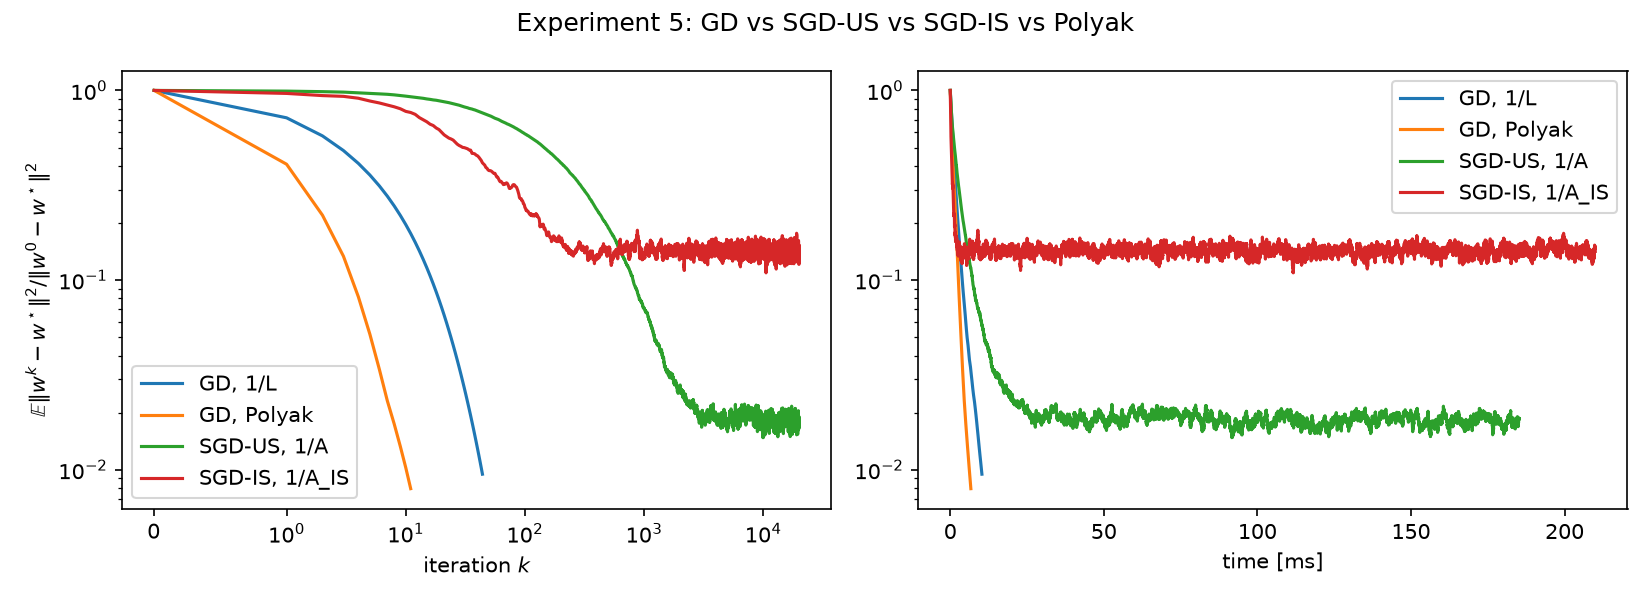
\includegraphics[width=\textwidth]{figures/log_exp5_comparison.png}
\end{center}

\end{document}
